%%%%%%%%%%%%%%%%%%%%%%%%%%%%%%%%%%%%%%%%%%%%
% En 'includes.tex' se encuentran la importación de paquetes necesarios
%%%%%%%%%%%%%%%%%%%%%%%%%%%%%%%%%%%%%%%%%%%%
%%%%%%%%%%%%%%%%%%%%%%%%%%%%%%%%%%%%%%%%%
% University Assignment Title Page 
% LaTeX Template
% Version 1.0 (27/12/12)
%
% This template has been downloaded from:
% http://www.LaTeXTemplates.com
%
% Original author:
% WikiBooks (http://en.wikibooks.org/wiki/LaTeX/Title_Creation)
%
% License: CC BY-NC-SA 3.0 (http://creativecommons.org/licenses/by-nc-sa/3.0/)
% 
% Instructions for using this template:
% This title page is capable of being compiled as is. This is not useful for 
% including it in another document. To do this, you have two options: 
%
% 1) Copy/paste everything between \begin{document} and \end{document} 
% starting at \begin{titlepage} and paste this into another LaTeX file where you 
% want your title page.
% OR
% 2) Remove everything outside the \begin{titlepage} and \end{titlepage} and 
% move this file to the same directory as the LaTeX file you wish to add it to. 
% Then add \input{./title_page_1.tex} to your LaTeX file where you want your
% title page.
%
%%%%%%%%%%%%%%%%%%%%%%%%%%%%%%%%%%%%%%%%%
%\title{Title page with logo}
%----------------------------------------------------------------------------------------
%	PACKAGES AND OTHER DOCUMENT CONFIGURATIONS
%----------------------------------------------------------------------------------------
\PassOptionsToPackage{warn}{textcomp}
\documentclass[14pt]{extarticle}
%Paquetes para idioma español y codifcación UTF8
\usepackage[spanish]{babel}
\usepackage[utf8]{inputenc}
\usepackage{csquotes}

%%% BIBLATEX
\usepackage{biblatex}
%%% BIBLIOGRAPHY
\addbibresource{references.bib}

%fuente 'fourier'
\usepackage{fourier}
%paquete para URLs
\usepackage{url}
\usepackage[hidelinks]{hyperref}
%paquete para ubicar las imágenes
\usepackage{float}
%paquete para imágenes y en dónde las tiene que buscar
\usepackage{graphicx}
\graphicspath{{images/}}
%paquete para epígrafes
\usepackage{subcaption}
%paquete para definir los márgenes de la hoja
\usepackage[left=1.5cm,right=1.5cm,top=3cm,bottom=3cm]{geometry}
%paquete para poner todos y comentarios
\usepackage[colorinlistoftodos]{todonotes}
%paquete para trabajar con código
\usepackage{listings}
%paquete para trabajar con colores y definir propios
\usepackage{color}

%paquete para el checkmark y la cruz
\usepackage{pifont}
%paquete para el signo de copyright
\usepackage{textcomp}

%paquete para que los \texttt{} no rompan el margen de la página
\usepackage[htt]{hyphenat}

\usepackage{enumerate}
%paquete para armar layouts multicolumna
\usepackage{multicol}


%Cabeceras
\usepackage{fancyhdr}
\pagestyle{fancy}
\fancyhead[L]{Administración de Redes y Seguridad, 2018}
\fancyhead[C]{}
\fancyhead[R]{UNPSJB}

\fancyfoot[R]{Luciano Serruya Aloisi}

%Comando para poner doble comillas más fácil
\newcommand{\dq}[1]{``#1''}
\newcommand{\cmark}{\ding{51}}
\newcommand{\xmark}{\ding{55}}

\definecolor{comment-green}{rgb}{0,0.5,0}
\definecolor{bg-light-gray}{HTML}{E9E9E9}
\definecolor{bg}{HTML}{D0B698}

\lstdefinestyle{bashstyle}{
    language=Bash,
    backgroundcolor=\color{bg},
    basicstyle=\ttfamily,
  	keywordstyle=\bfseries\color{white},
    stringstyle=\color{blue},
    commentstyle=\color{comment-green}\itshape,
    numberstyle=\color{gray},
    identifierstyle=\color{black},
    rulecolor=\color{gray},
    showstringspaces=false,
    escapeinside={\%*}{*)},
    morekeywords={},
    otherkeywords={},
    breaklines=true,
    frame=trbl, 
    framexleftmargin=25pt,
    numbers=left,
    xleftmargin=\parindent,
    frameround=tttt,
    captionpos=b,
    % re tirado de los pelos, pero es lo que hay
    % sacado de:
    % https://tex.stackexchange.com/questions/24528/having-problems-with-listings-and-utf-8-can-it-be-fixed
    inputencoding=utf8,
    extendedchars=true,
    literate={á}{{\'a}}1 {é}{{\'e}}1 {í}{{\'i}}1 {ó}{{\'o}}1 {Ó}{{\'O}}1 {ú}{{\'u}}1,
}



\begin{document}

%%%%%%%%%%%%%%%%%%%%%%%%%%%%%%%%%%%%%%%%%%%%
% En 'titlepage.tex' se encuentra la página de título
%%%%%%%%%%%%%%%%%%%%%%%%%%%%%%%%%%%%%%%%%%%%
\begin{titlepage}

    \newcommand{\HRule}{\rule{\linewidth}{0.5mm}} % Defines a new command for the horizontal lines, change thickness here

    \center % Center everything on the page
     
    %----------------------------------------------------------------------------------------
    %	HEADING SECTIONS
    %----------------------------------------------------------------------------------------

    \textsc{\LARGE UNPSJB}\\[1cm] % Name of your university/college
    \textsc{\Large Licenciatura en Sistemas OPGCPI}\\[0.5cm] % Major heading such as course name
    \textsc{\large Administración de Redes y Seguridad}\\[0.5cm] % Minor heading such as course title

    %----------------------------------------------------------------------------------------
    %	TITLE SECTION
    %----------------------------------------------------------------------------------------

    \HRule \\[0.4cm]
    {\huge \bfseries Trabajo Práctico 1}\\[0.4cm] % Title of your document
    {\large \bfseries Concientización}\\[0.4cm] % Title of your document
    \HRule \\[1.5cm]
     
    %----------------------------------------------------------------------------------------
    %	AUTHOR SECTION
    %----------------------------------------------------------------------------------------


    \begin{minipage}[l]{0.5\textwidth}
        \begin{flushleft}
            \textbf{\textsf{Cátedra}}\\
            \large Lic. Bruno Damián Zappellini\\ 
            \linespread{4}
            \end{flushleft}
    \end{minipage}
    \begin{minipage}[l]{0.4\textwidth}
        \begin{flushright}
            \textbf{\textsf{Integrantes:}}\\
            \linespread{1}
            \large Luciano Serruya Aloisi\\
        \end{flushright}
    \end{minipage}\\[1.5cm]

    % If you don't want a supervisor, uncomment the two lines below and remove the section above
    %\Large \emph{Author:}\\
    %John \textsc{Smith}\\[3cm] % Your name

    %----------------------------------------------------------------------------------------
    %	DATE SECTION
    %----------------------------------------------------------------------------------------

    {\large \today}\\[1cm] % Date, change the \today to a set date if you want to be precise

    %----------------------------------------------------------------------------------------
    %	LOGO SECTION
    %----------------------------------------------------------------------------------------

    
\includegraphics[scale=1]{logoUnpsjb.png}\\[0.5cm] % Include a department/university logo - this will require the graphicx package
     
    %----------------------------------------------------------------------------------------

    % \vfill % Fill the rest of the page with whitespace

\end{titlepage}


%%%%%%%%%%%%%%%%%%%%%%%%%%%%%%%%%%%%%%%%%%%%
% INDICE
%%%%%%%%%%%%%%%%%%%%%%%%%%%%%%%%%%%%%%%%%%%%
\clearpage
\tableofcontents
\clearpage 

\lstset{style=bashstyle}

\section{Conceptos básicos}

\emph{Juan quiere mandarle un mensaje a Julio. A Julio no le importa asegurarse que el mensaje fue enviado por Juan, sin embargo Juan quiere estar seguro de que el mensaje no podra ser leído ni alterado por un tercero. Juan trabaja en una empresa en Argentina y Julio es empleado de una empresa ubicada en España} 

Para esta situación, un sistema de cifrado simétrico no cumpliría los requisitos solicitados; en el caso de que la clave compartida sea interceptada, la comunicación puede ser espiada por un tercero. Sin embargo, si se garantiza un canal seguro para transmitir la clave privada al inicio de la comunicación, sí se podría utilizar un cifrado simétrico. En caso de que esto último no sea posible, la alternativa sería usar un sistema de cifrado asimétrico, donde el emisor encripta el mensaje con la clave pública del receptor, y el receptor desencripta el mensaje recibido con su clave privada.

\vspace*{5mm}
\emph{Adriana y Leandro quieren comunicarse en forma segura. Para ellos resulta facil conseguir un medio seguro para intercambiar informacion que luego necesiten para realizar esta comunicacion segura. En este caso lo que importa es que nadie pueda espiar los datos involucrados en dicha comunicación} 
~\\

Debido a que se cuenta con un canal seguro, se lo podría utilizar para compartir una clave, la cual se utilizará para cifrar los mensajes intercambiados de forma simétrica.

\vspace*{5mm}
\emph{Analía usara el correo electrónico para enviar la aceptación de un contrato al estudio en el cual trabaja. Para la persona que lo reciba es importante tener la garantía de que el mismo fue enviado efectivamente por Analía} 

Lo adecuado para esta situación sería que el correo enviado por Analía sea firmado utlizando la clave privada de Analía.

\vspace*{5mm}
\rule{.9\linewidth}{0.3mm}

\subsection{Verdadero o falso}

\emph{En los criptosistemas simétricos no puede garantizarse el no repudio porque ambas partes de la transacción conocen la clave utilizada} 

\textbf{Falso}. Si la clave compartida no fue transmitida por un canal seguro puedo haber sido interceptada, logrando que un tercero envíe un mensaje encriptado. 

\vspace*{5mm}
\emph{Si únicamente me importara la eficiencia del método que uso para encriptar, debería optar por un algoritmo de cifrado asimétrico} 

\textbf{Falso}. Si se busca eficiencia, la encriptación asimétrica se debería evitar. La encriptación simétrica es mucho más rápida y no incrementa el tamaño del mensaje. 

\vspace*{5mm}
\emph{Con ambos tipos de criptosistemas necesito contar con un mecanismo seguro para transmitir la clave} 

\textbf{Falso}. Con los criptosistemas asimétricos, no es necesario que las claves públicas sean compartidas de forma segura (se pueden alojar en un servidor o un repositorio para que disintios usuarios la consigan).

\section{\emph{PKI}}

Para poder verificar la firma de un correo eletrónico, el receptor necesita la \textbf{clave pública} del emisor. 

Al enviar un mensaje firmado, el emisor genera un \emph{resumen} del mensaje (con alguna función de \emph{hashing}), y luego lo encripta con su \textbf{clave privada}, generando así la \textbf{firma digital}. 

El receptor también genera el resumen del mensaje (con el mismo algoritmo), y desencripta la firma con la \textbf{clave pública} del emisor (el receptor debía contar con la clave pública del emisor o la debe poder conseguir ya sea a través de un \emph{certificado} o de un repositorio). Luego compara el resumen que él generó, y el que recibió del emisor. Si son iguales, entonces la firma es considerada válida; si no son iguales, entonces significa que se utilizó una clave distinta para firmar el mensaje, o fue alterado.

Ahora bien, si el mensaje está encriptado, para poder abrirlo el receptor necesita su \textbf{clave privada}, ya que el mensaje debió ser cifrado con la \textbf{clave pública} del receptor. En caso de que el mensaje hubiese sido cifrado con la \textbf{clave privada} del emisor, cualquier tercero que tenga la \textbf{clave pública} del emisor podrá desencriptarlo.

\subsection{Instalando un certificado en Firefox}

\begin{itemize}
    \item Algoritmo de firma utilizado: \texttt{PKCS \#1 MD5 With RSA Encryption} 
    \item Cantidad de bits de cifrado: \texttt{4096 bits} 
    \item Periodo de validez: desde el \texttt{30/03/2003} hasta el \texttt{29/03/2033} 
    \item Emisor:
    \begin{itemize}
        \item E = support@cacert.org
        \item CN = CA Cert Signing Authority
        \item OU = http://www.cacert.org
        \item O = Root CA
    \end{itemize}
\end{itemize}

\begin{figure}[h]
    \centering
    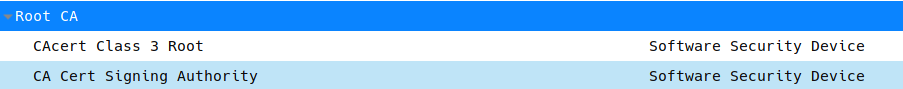
\includegraphics[width=\linewidth]{images/arys-tp3-cacert-certificado-instalado.png}
    \caption*{Certificado de CACert instalado en Firefox}
\end{figure}

\begin{figure}[h]
    \centering
    
\includegraphics{images/arys-tp3-cacert-con-https.png}
    \caption*{Ingresando a CACert con HTTPS}
\end{figure}

\subsection{Certificado personal}

Después de generar el certificado personal para la dirección de correo electrónico \emph{lucianoserruya@gmail.com} e instalarlo en Firefox, se puede ver el siguiente certificado instalado 

\begin{figure}[H]
    \centering
    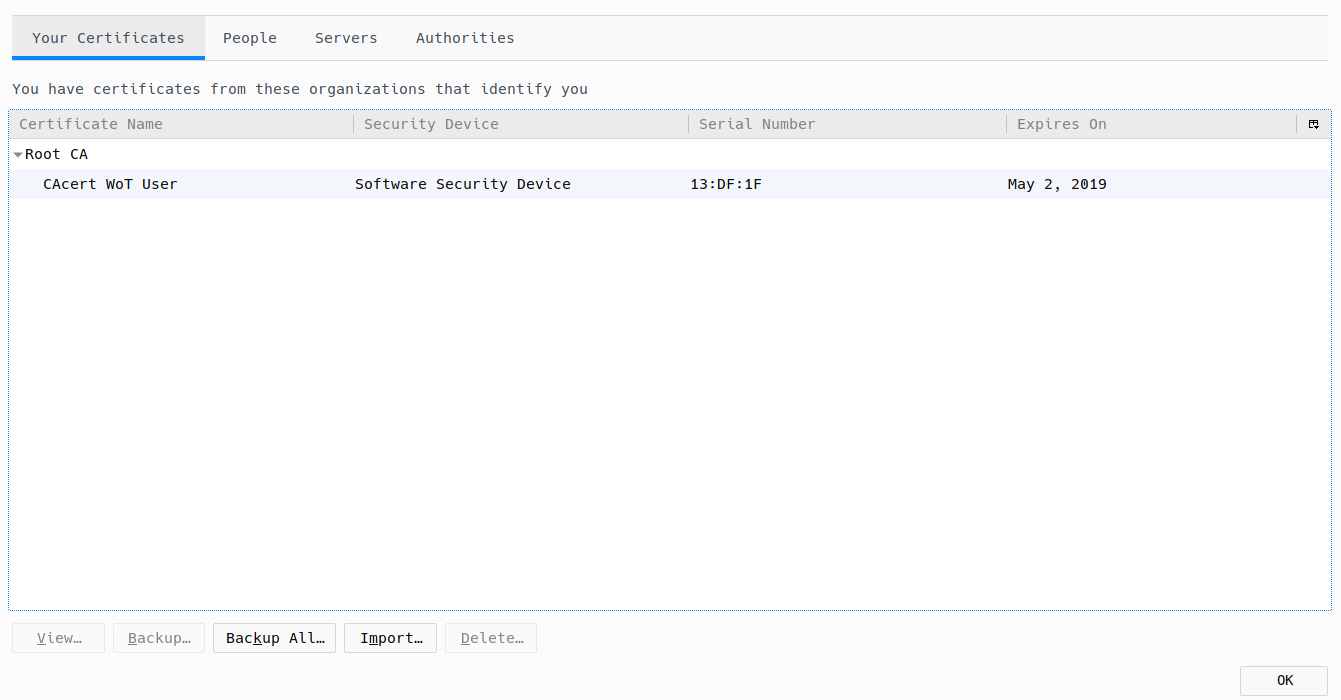
\includegraphics[width=\linewidth]{images/arys-tp3-cacert-certificado-gmail.png}
    \caption*{Certificado personal instalado en Firefox}
\end{figure}

\subsection{Correos electrónicos firmados y encriptados}

\emph{Para los siguientes experimentos que se muestran a continuación, se utilizaron dos cuentas personales: \emph{lucianoserruya@gmail.com} y \emph{lucianoserruya@hotmail.com}. Para ambas cuentas se generaron los respectivos certificados en CACert y se instalaron correctamente en Thunderbird} 

\vspace*{5mm}

Una vez instalados los certificados de ambas cuentas en Thunderbird, se realizaron los siguientes experimentos:

\begin{itemize}
    \item Enviar un correo firmado - el emisor necesita su clave privada para encriptar la firma, y el receptor necesita la clave pública del emisor para poder verificarla
    \item Enviar un correo encriptado - el emisor necesita la clave pública del receptor para encriptar el mensaje, y el receptor necesita su clave privada para poder desencriptarlo
    \item Enviar un correo firmado y encriptado - se tienen que cumplir las dos condiciones anteriores
\end{itemize}

A continuación se incluyen capturas de pantalla de los correos electrónicos enviados. Como el mismo cliente tiene tanto las claves privadas como las públicas de ambas cuentas, se pudieron realizar los experimentos sin incovenientes.

Thunderbird indica con un logo de un candado a los correos que hayan sido encriptados, y con un sobre a aquellos que fueron firmados (y que se pudo validar la firma).

\begin{figure}[h]
    \centering
    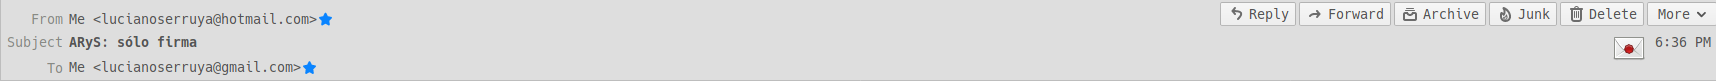
\includegraphics[width=\linewidth]{images/arys-tp3-correo-firmado.png}
    \caption*{Correo firmado}
\end{figure}

\begin{figure}[h]
    \centering
    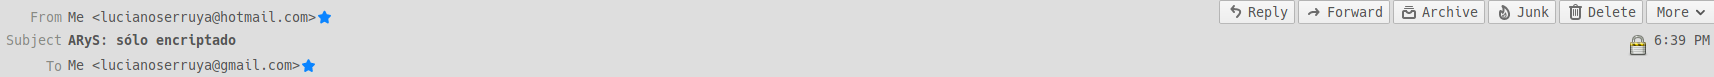
\includegraphics[width=\linewidth]{images/arys-tp3-correo-encriptado.png}
    \caption*{Correo encriptado}
\end{figure}

\begin{figure}[h]
    \centering
    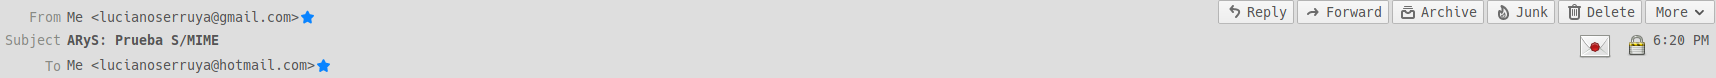
\includegraphics[width=\linewidth]{images/arys-tp3-correo-firmado-encriptado.png}
    \caption*{Correo firmado y encriptado}
\end{figure}



\subsection{Análisis sobre una clave privada robada}

La infraestructura de PKI brinda un elemento esencial una situación de este tipo. Este se llama \textbf{\emph{Certificate Revocation List} (\emph{CRL})}, es un repositorio que mantiene la \emph{CA} (\emph{Certificate Authority}, ente encargado de emitir los certificados) con los certificados que dejaron de ser válido (que fueron revocados, los certificados expirados no entran en esta lista). 

\subsubsection{Cómo actuar}

Tanto si la clave privada fue robada como si fue robada y además eliminada de la máquina del dueño, lo primero que se debe hacer es \textbf{revocar los certificados} que corresponden a esa clave privada. Para ello se debe agregar el número de identificación del certificado a la \emph{CRL} de la \emph{CA} correspondiente.  

Cuando un cliente pida el certificado del servidor cuya clave privada fue comprometida, lo rechazará y pedirá uno nuevo al verificar que ese certificado se encuentra en la \emph{CRL}. 

\subsubsection{Consecuencias con la información encriptada}

Como la clave privada es la que usa utiliza para desencriptar mensajes, estando comprometida un tercero podría desencriptar los mensajes que vayan hacia el dueño original de la clave.

\subsubsection{Consecuencias con la información firmada}

Para firmar se utiliza la clave privada, por lo tanto alguien más podría firmar documentos haciéndose pasar por el dueño de la clave.


\section{\emph{PGP}}

\emph{Al igual que en la sección anterior, para las pruebas de firmar y encriptar correos electrónicos con PGP, se utilizaron las mismas cuentas} 

\vspace*{5mm}

\subsection{Crear claves \emph{PGP} con \texttt{gpg}}

Para crear las claves PGP utilizando la aplicación de línea de comando \texttt{gpg}, se debe ejecutar el siguiente comando:

\begin{lstlisting}
gpg --gen-key 
\end{lstlisting}

A continuación se detallan los datos que son requeridos por la aplicación para crear el par de claves

\begin{itemize}
    \item Algoritmos de encriptación
    \item Tamaño (en bits) de la clave
    \item Tiempo máximo de validez de la clave
    \item Nombre real/nombre de usuario
    \item Dirección de correo electrónico
    \item Comentario
\end{itemize}

\begin{figure}[H]
    \centering
    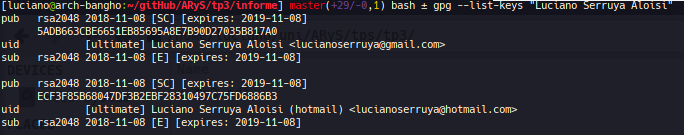
\includegraphics[width=\linewidth]{images/arys-tp3-gpg-claves-publicas.png}
    \caption*{Claves públicas PGP}
\end{figure}

Una vez creado el par de claves, a través del complento de Thunderbird, \emph{Enigmail}, se pueden cargar al cliente de correo para poder encriptar y firmar los correos con estas claves

\begin{figure}[H]
    \centering
    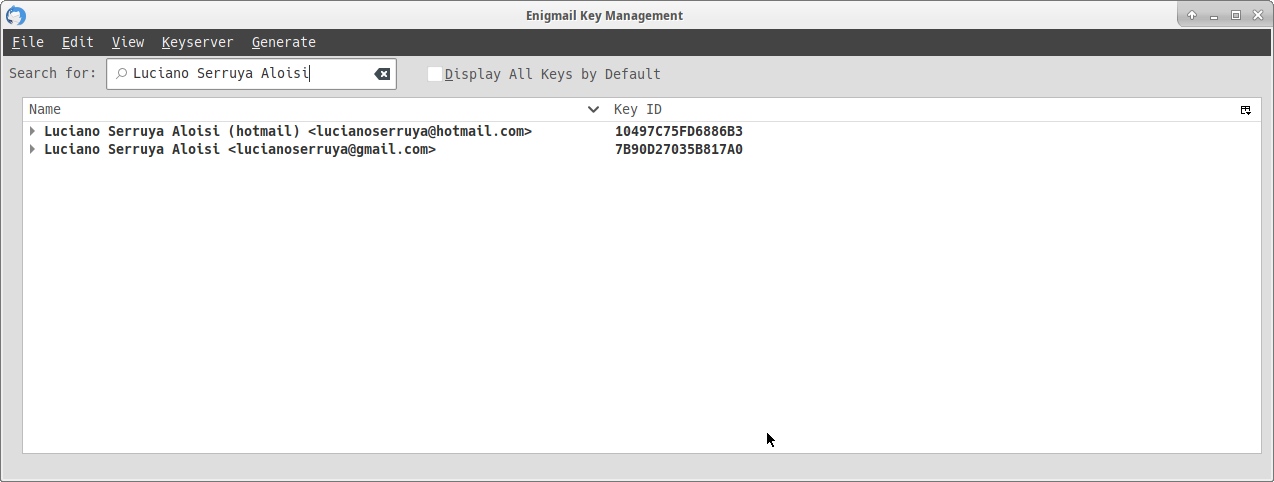
\includegraphics[width=\linewidth]{images/arys-tp3-claves-pgp-thunderbird.png}
    \caption*{Claves públicas cargadas en Thunderbird}
\end{figure}

\subsubsection{Prueba de correo firmado y encriptado}

A continuación se muestran capturas de un correo electrónico firmado y encriptado con PGP, enviado desde la cuenta \emph{lucianoserruya@hotmail.com} a la cuenta \emph{lucianoserruya@gmail.com}.

\begin{figure}[H]
    \centering
    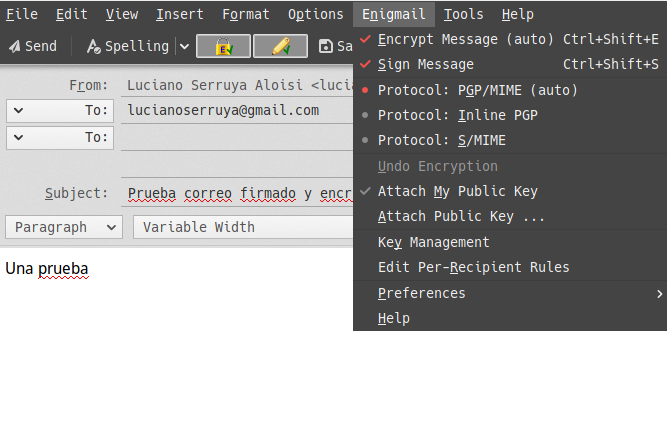
\includegraphics[width=\linewidth]{images/arys-tp3-correo-firmado-encriptado-pgp.png}
    \caption*{Enviado correo firmado y encriptado}
\end{figure}

\begin{figure}[H]
    \centering
    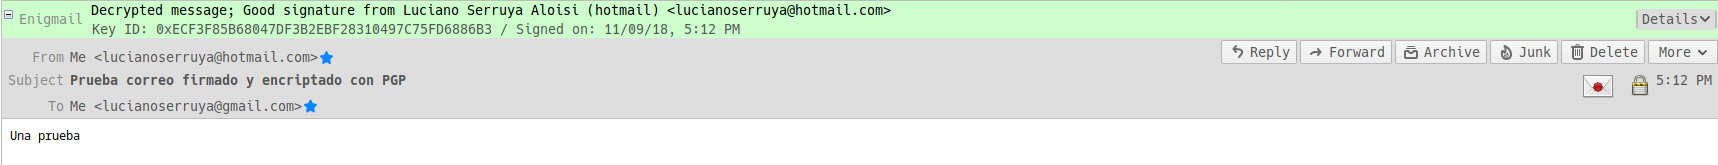
\includegraphics[width=\linewidth]{images/arys-tp3-correo-recibido-firmado-encriptado-pgp.png}
    \caption*{Correo recibido correctamente}
\end{figure}


\subsection{Relaciones de confianza}

Una vez importadas las claves de las cuentas \emph{bruno.zappellini@gmail.com} y \emph{bzappellini@juschubut.gov.ar}, el estado de validez de las claves es el siguiente:

\begin{figure}[H]
    \centering
    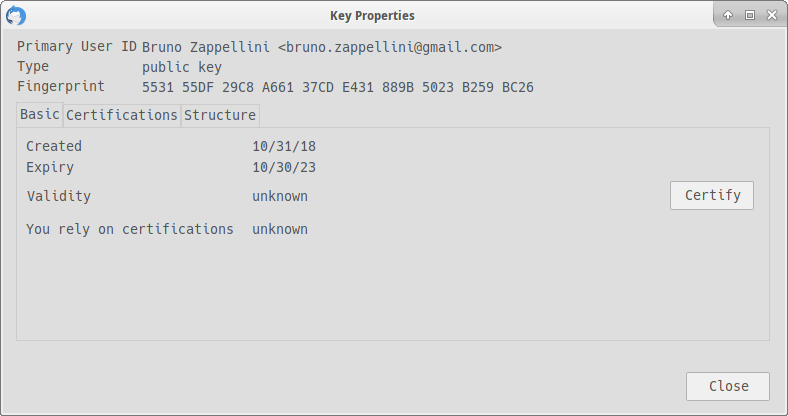
\includegraphics[width=.8\linewidth]{images/arys-tp3-clave-pgp-gmail-zape.png}
    \caption*{Clave para \emph{bruno.zappellini@gmail.com}}
\end{figure}

\begin{figure}[H]
    \centering
    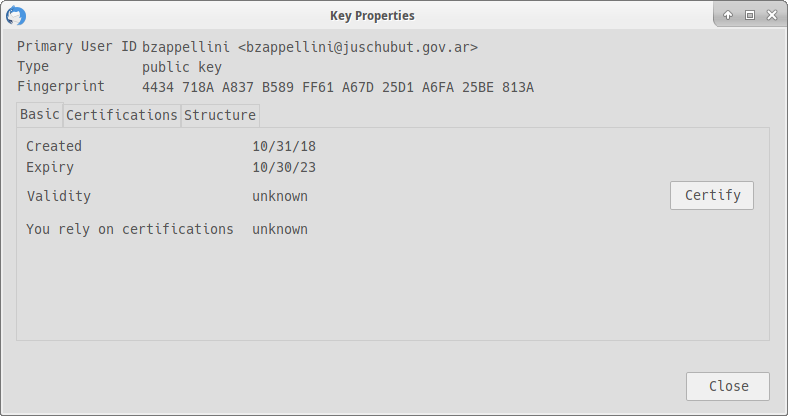
\includegraphics[width=.8\linewidth]{images/arys-tp3-clave-pgp-juschubut-zape.png}
    \caption*{Clave para \emph{bzappellini@juschubut.gov.ar}}
\end{figure}

Ahora bien, como la segunda clave está firmada por la primera, si se certifica que la primera es de quién dice ser (con la opción \texttt{Certify} en Thunderbird), la segunda automáticamente también estaría certificada. Este compartamiento se debe al \emph{\textbf{modelo de confianza}} de PGP.

\begin{figure}[H]
    \centering
    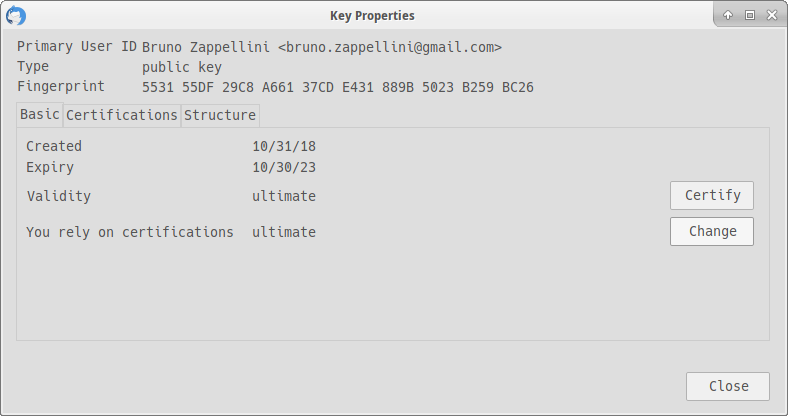
\includegraphics[width=0.8\linewidth]{images/arys-tp3-clave-pgp-gmail-zape-confiada.png}
    \caption*{Clave para \emph{bruno.zappellini@gmail.com} certificada - \emph{se le concedieron los máximos niveles de confianza}}
\end{figure}

\begin{figure}[H]
    \centering
    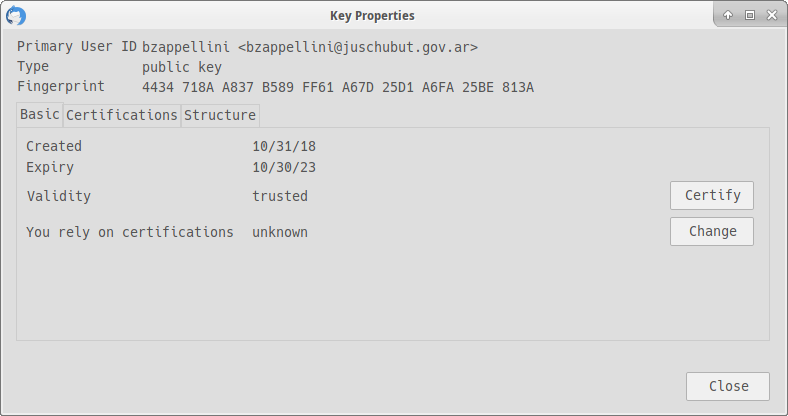
\includegraphics[width=0.8\linewidth]{images/arys-tp3-clave-pgp-juschubut-zape-confiada.png}
    \caption*{La clave para \emph{bzappellini@juschubut.gov.ar} es validada automáticamente por el \emph{modelo de confianza}}
\end{figure}

\subsubsection{Cambiando confianza de las claves}

Al recibir un correo de la cuenta \emph{bruno.zappellini@gmail.com} teniendo la clave PGP sin verificar, el cliente Thunderbird indica que se pudo verificar la firma digital, pero muestra una salida distinta

\begin{figure}[H]
    \centering
    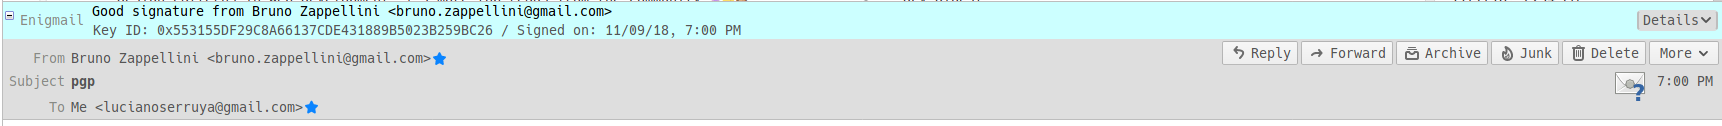
\includegraphics[width=\linewidth]{images/arys-tp3-clave-pgp-sin-verificar.png}
    \caption*{Clave PGP sin verificar}
\end{figure}

Ahora bien, si verificamos que la clave es de su dueño, certificándolo con nuestra clave privada, Thunderbird muestra la firma de otra manera

\begin{figure}[H]
    \centering
    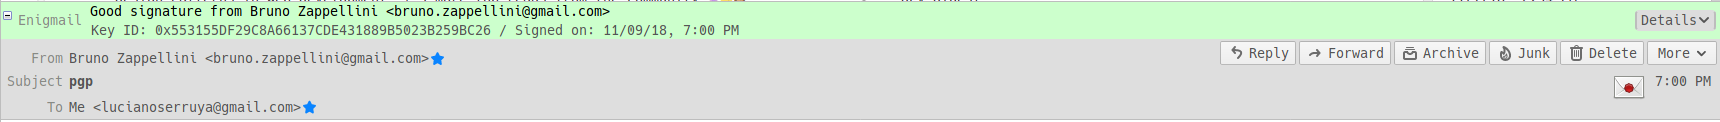
\includegraphics[width=\linewidth]{images/arys-tp3-clave-pgp-verificada.png}
    \caption*{Clave PGP verificada con nuestra clave privada}
\end{figure}

\subsection{Mecanismo de firma y encriptación con PGP}

PGP al ser un sistema de encriptación \textbf{asimétrico}, utiliza la \textbf{clave privada} para firmar los documentos, y la \textbf{clave pública del receptor} para encriptarlos.   

\subsection{Situaciones de confianza de una clave}

Un cliente de correo (como Thunderbird, por ejemplo) puede confiar en una clave PGP (que no sea nuestra) por alguna de las siguientes razones:

\begin{itemize}
    \item El usuario explícitamente decidió confiar en dicha clave (firmando la misma) - relación de confianza \textbf{directa} 
    \item Se puede establecer una relación de confianza \textbf{indirecta}
    \begin{itemize}
        \item El dueño de alguna clave de la cual confiamos plenamente (confianza \emph{FULL}) firmó la clave
        \item La clave fue firmada por \emph{X} claves en las que confiamos marginalmente (confianza \emph{MARGINAL}) 
    \end{itemize}
\end{itemize}


\subsection{Análisis sobre una clave privada robada}

PGP permite \textbf{revocar} claves a través de \textbf{certificados de revocación de claves}, ya sea porque se cambió de clave o porque la clave privada fue comprometida. 

Cuando una clave es revocada, PGP debe contactar a los servidores en los cuales esté alojada la clave pública para actualizar su estado. De esta forma, cuando otros usuarios quieran actualizar la clave pública desde el servidor, estos se enterarán que está revocada.

Ahora bien, para generar el certificado de revocación se necesita tanto la \textbf{clave privada}, como su \textbf{contraseña}. 

\subsubsection{Cómo actuar}

Si la clave privada fue comprometida \textbf{pero todavía está presente en la máquina del dueño}, se puede generar un certificado de revocación para revocarla.

Si la clave privada fue comprometida y eliminada de la máquina del dueño, \textbf{no hay nada que se pueda hacer}; se necesitan las dos partes (la clave privada y su contraseña) para generar el certificado de revocación. 

\subsubsection{Consecuencias con la información encriptada}

Aquel que posea la clave privada podrá desencriptar la información que iba encriptada para el dueño original.

\subsubsection{Consecuencias con la información firmada}

El usuario que tenga la clave privada podrá firmar correos haciéndose pasar por el dueño original.



\section{Criptografía simétrica y esteganografía}

\subsection{Encriptando archivos con \texttt{gpg}}

La aplicación \texttt{gpg} permite generar pares de claves asimétricas PGP y también permite encriptar \textbf{simétricamente} un archivo; según las páginas \texttt{man}, el algoritmo por defecto para encriptación simétrica es  \textbf{AES-128} (se puede cambiar utilizando el parámetro \texttt{--cipher-algo}).   

Se puede crear un nuevo archivo y encriptarlo con \texttt{gpg} de la siguiente manera

\begin{lstlisting}
echo "Un mensaje secreto" > secreto.txt
gpg -c secreto.txt
\end{lstlisting}

La aplicación levantará una ventana para ingresar una contraseña, y luego confirmarla; con dicha clave se encriptará el archivo de forma simétrica.

\begin{figure}[H]
    \centering
    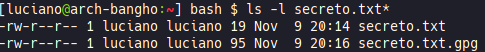
\includegraphics[width=\linewidth]{images/arys-tp3-pgp-simetrico.png}
    \caption*{Archivo encriptado y no encriptado - el archivo encriptado es considerablemente mayor}
\end{figure}

Para desencriptarlo, sencillamente se debe ejecutar el comando

\begin{lstlisting}
gpg -d secreto.txt.gpg > secreto_desencriptado.txt
\end{lstlisting}

Ingresar la contraseña con la que se encriptó el mensaje.




%%%%%%%%%%%%%%%%%%%%%%%%%%%%%%%%%%%%%%%%%%%%
% FIN DOCUMENTO, AHORA REFERENCIAS
%%%%%%%%%%%%%%%%%%%%%%%%%%%%%%%%%%%%%%%%%%%%
\clearpage
\printbibliography

\end{document}
